\chapter{先行研究}
\begin{figure}[ht]
    \centering
    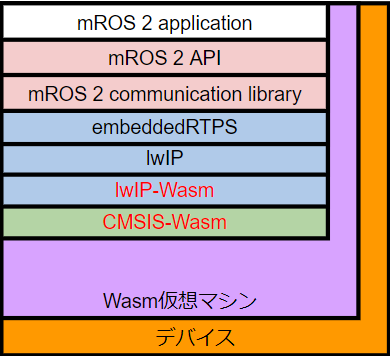
\includegraphics[width=10cm]{images/fig3_mros2-wasm_configuration.png}
    \caption{mROS2-wasmの構成図}
    \label{fig:mros2-wasm_configuration}
\end{figure}
柿本らによって,mros2-POSIXをwasm環境で実行するmros2-wasmが提案された.[]
WebAssembly(Wasm)は,C,C++,C\#,Rustなどの言語で書かれたプログラムをコンパイルのターゲットWeb上でプログラムを高速に実行するために設計された,スタックベースの仮想マシンで実行される仮想命令アーキテクチャである.[4][16]
サンドボックスな環境でアプリケーションは実行されるため,ハードウェアや言語,プラットフォームに依存せず,ネイティブ日回実行速度でコードを実行できるという性質がある[]
Wasmの性質からWebブラウザ以外の実行環境として利用する取り組みがあり,Webの外部でWasmを実行するためのAPI群としてWASI(WebAssembly System Interface)[]が提案された.WASIを用いることでファイルやディレクトリ,ネットワークソケットなど,様々なリソースにWasmからアクセスできるようになり,Webブラウザ以外の実行環境として動作するWasmランタイムの開発が進んだ.
\\ mROS2をWasm化させるにともない,使用するWasmランタイムに関して以下の制約がある.
\begin{itemize}
    \item ROSランタイムにはスレッド操作やネットワーク通信の処理が必要であるため,Wasmランタイムにはこれらの機能が必要である
    \item リソースの限られているエッジデバイスで動作させることを想定する必要があるため,WasmランタイムとROSランタイムによるリソース消費を最小限に抑える必要がある
\end{itemize}
これらの制約を満たすランタイムとしてWAMR(WebAssembly Micro Run-time)[]がある.
WAMRは,組込みやIoT,クラウドなど,様々なプラットフォームで動くようにメモリ消費量が小さくなるよう設計された,オープンソースのWasmランタイムである.Wasmプログラムの実行方式としてはWasmバイナリを逐次実行するインタプリタ方式と(Classic),事前にWasmバイナリをネイティブバイナリにコンパイルして実行するAoT(Ahead Of Time),Wasmバイナリをネイティブバイナリにコンパイルして実行するJIT(Just In Time)があり,そのうちAoTとJITではネイティブと同等の実行速度で動作する.またマルチスレッドやスレッド管理を行うpthread API(POSIXスレッドの標準API)をサポートする組込みライブラリやSocket APIをサポートする組込みライブラリも提供されている.\\ Wasmはサンドボックスな環境で実行されるため,OSの機能に依存した層があるmROS 2-POSIXをそのままではコンパイルすることができない.
図2.2で示したとおり,mROS 2-POSIXでOSに依存している層はCMSIS-POSIXとlwIP-POSIXである.
CMSIS-POSIXはmROS 2内部でRTPS通信を行うための機能として,スレッド管理機能,排他制御機能,メッセージキュー管理機能,時間管理機能がpthreadなどを用いて実装されている.lwIPでは,UDPマルチキャストをおこなための実装がSocketやCMSIS-POSIXが提供する機能を用いて実装されている.
\\ これらの依存を解消するため,CMSIS-POSIXをWasm対応したCMSIS-WASM,lwIP-POSIXをWasm対応したlwIP-WASMを柿本らは実装した.
mROS2-wasmの構成を図3.1に示す.
なお,mROS 2はオープンソースソフトウェアであることから上位レイヤに変更が加わっても変更を取り込みやすいよう,既存のビルドシステムに極力手を加えずにシステムを構築されている.
\\ CMSIS-WASMを実装する機能のうち,排他制御機能,メッセージキュー管理機能はスレッド管理機能に依存している.時間管理機能は手を加えることなくWasmコンパイルが可能であったため,実際に実装されたのはスレッド管理機能である.
実装に際して,WAMRのpthread APIを用いてスレッド管理機能を実装されているがWAMR pthread ライブラリの既知の問題が障害となった.
\begin{itemize}
    \item timespec 構造体をサポートしていない
    \item wasi-sysrootのerrnoと互換性がない
    \item pthread\_attr\_t 構造体をサポートしていない
\end{itemize}
timespec構造体は,スレッドの同期処理などに使われるpthread\_cond\_timedwait 関数から使用され,待機時間の長さを指定するために使われる.WAMRではtimespec構造体が使われず,usecondsを用いる必要があった.そのため待機死体時間をマイクロ秒単位に変換し引数としてWAMRのpthread\_cond\_timewaitに渡すことでtimespec構造体を用いずに同様の動作をさせた.
\\ errnoに関してはシステムが正常に動作している際に使われることがないため,仕様が避けられている.
\\ スレッド生成時にそのスレッドの属性を設定するのに使われるpthread\_attr\_t構造体は,WAMRではサポートされていない.しかし,pthread\_attr\_tはスレッドを生成する関数のみで使用されており,デフォルトの属性から変更されずにスレッド適用されていたため,削除されている.CMSIS-WASMは上記のように柿本らによって実装された.
\\ lwIP-WASMは,Socketを用いて通信機能の実装が行われているため,WASIを用いる必要がある.WAMRにはWASIを用いて実装されたSocket APIが提供されているため,それを用いて実装が行われた.
\\ WAMRのSocket APIでは,setsockopt関数においてIPPROTO\_IPレベル()で設定できるオプションは5つに限られている.
\begin{itemize}
    \item IP\_MULTICAST\_LOOP
    \item IP\_ADD\_MEMBERSHIP
    \item IP\_DROP\_MEMBERSHIP
    \item IP\_TTL
    \item IP\_MULTICAST\_TTL
\end{itemize}
一方,mROS 2-POSIXのlwIP-POSIXでは,IP\_MULTICAST\_IF,IP\_ADD\_MEMBERSHIP,IP\_MULTICAST\_TTLが使用されており,IP\_MULTICAST\_IFがWAMRのSocket APIには存在しないためネットワークインターフェースの指定ができないという問題があった.SocketはIP\_MULTICAST\_IFによるネットワークインターフェースの指定がない場合はデフォルトのネットワークインターフェースが指定されるため,IP\_MULTICAST\_IFを設定するsetsockopt関数を削除して実装が行われた.また,マルチキャスト通信の配信範囲を制御するTTLを設定するIP\_MULTICAST\_TTLの指定時に,WAMRのSocket APIではオプションデータの長さが4bytesでないときプログラムが終了してしまう.lwIP-POSIXではこの長さが1bytesで定義されていたため4bytesに変更した.このようにWAMRのSocket APIに合わせた細かい変更を行うことで,lwIP-WASMが実装された.
システムのビルドは,外部のプロジェクトのビルド・インストールなどを可能にするExternalProjectを用いてmROS 2のディレクトリ外から行うことができる.
\\ 以上の実装により,実行中のmROS 2-POSIXをWasm化することができた.
\\ mROS 2-Wasmは通信時間とメモリサイズと計算処理性能の評価が行われた.
\\ 計算処理性能の評価では,ノード内で擬似作業として1以上の整数を順に素数判定し,1024までの素数を見つける処理を行う実装をし,その時間を計測,評価した.
コンパイル方式はAoTとClassic インタプリタとFast インタプリタを使って計測した.
\\ 通信時間ではmROS 2-WasmとmROS 2を比較評価した.
計測方法はクラウド想定のデバイスから文字列データを送信し,ロボット想定のデバイスからデータを受けとると,そのままデータを返し,クラウド想定のデバイスが受け取るまでの時間,RTT(Round Trip Time)を計測している.mROS 2-Wasmのコンパイル方式はAoTとJITを使わずClassicインタプリタでコンパイルしたバイナリファイルを使って計測した.
\\ メモリサイズの評価では,mROS 2-POSIXとmROS 2-WasmとmROS 2-POSIXを比較評価している.この計測では,計算処理性能で実装された処理のプロセスIDのRSS(Resident Set Size)とVSS(Virtual Set Size)を取得し評価をした.
今後の課題として,mROS 2-Wasmに実行状態の保存,復元機構を実装することが残った.
%柿本さんの研究の評価方法を載せたい通信性能でAOTとJITは動作しなかったため,Classicでの評価が行われた.ということを言わないといけない